\documentclass[10pt,twocolumn,letterpaper]{article}

\usepackage{cvpr}
\usepackage{times}
\usepackage{epsfig}
\usepackage{graphicx}
\usepackage{amsmath}
\usepackage{amssymb}
\usepackage{algpseudocode}% http://ctan.org/pkg/algorithmicx
\usepackage{algorithm}% http://ctan.org/pkg/algorithm
\usepackage{subfig} %for subfigure environment
\usepackage{multirow}
\usepackage{array}
\usepackage{url}
\usepackage{bbm}


\usepackage[normalem]{ulem}

\newcommand{\argmax}{\operatornamewithlimits{argmax}}
\newcommand{\argmin}{\operatornamewithlimits{argmin}}
\newcommand{\eqdef}{\overset{\mathrm{def}}{=\joinrel=}}


% Include other packages here, before hyperref.

% If you comment hyperref and then uncomment it, you should delete
% egpaper.aux before re-running latex.  (Or just hit 'q' on the first latex
% run, let it finish, and you should be clear).
\usepackage[pagebackref=true,breaklinks=true,letterpaper=true,colorlinks,bookmarks=false]{hyperref}

\cvprfinalcopy % *** Uncomment this line for the final submission

\def\cvprPaperID{118} % *** Enter the CVPR Paper ID here
\def\httilde{\mbox{\tt\raisebox{-.5ex}{\symbol{126}}}}

% Pages are numbered in submission mode, and unnumbered in camera-ready
\ifcvprfinal\pagestyle{empty}\fi
\begin{document}

%%%%%%%%% TITLE
\title{Interactive Action Recognition using Relative Geometry Between Body Parts}

\author{Swami Sankaranarayanan and Kota Hara\\
Center for Automation Research, University of Maryland, College Park, MD 20742\\
{\tt\small \{swamiviv,kotahara\}@umiacs.umd.edu}
% For a paper whose authors are all at the same institution,
% omit the following lines up until the closing ``}''.
% Additional authors and addresses can be added with ``\and'',
% just like the second author.
% To save space, use either the email address or home page, not both
}


\maketitle
%\thispagestyle{empty}

%%%%%%%%% ABSTRACT
\begin{abstract}
In this work, we propose
   
\end{abstract}

%%%%%%%%% BODY TEXT
\section{Introduction}

Action recognition from the body skeleton has been very active due to the advance of motion capture system such as Kinect. Action recognition systems use the skeleton information as an input to predict the action taking place. Typically the skeleton information is given in the form of 3d locations of a set of body joints. Many action recognition systems directly use these information as the input or convert the location information into a set of joint angles and then use them as the input. The focus of the research has been on the recognition part. 

\cite{Vemulapalli2013} proposed a new skeleton representation based on relative geometry across body parts and achieve the state of the art results on several standard action recognition dataset. They compute the translation and rotation between each pair of body parts and map it to the tangent space to get a feature vector. The benefit of their approach compared to the previously adopted skeleton representation is that their method capture the relationship between body parts that are not directly connected each other. Thus, their method is more capable of representing actions in which the relationship between non-connected body parts, such as left arm and right arm, is important.

In this work, our task is to classify action performed between two people. We also use relative geometry across body parts but unlike their work, we also consider relative geometry between body parts across two people. This representation enables us to capture two people's interaction well.


\section{Related Work}

\section{Action Localization}


\section{Skeleton Representation}





%\subsection{Special Euclidean Group and Quaternions}
%In this section, we briefly discuss the Special Euclidean Group $SE(3)$. The special Euclidean Group, $SE(3)$, is the Lie group of all 4 by 4 matrices of the form
%\begin{equation}
%P(R,\vec{d}) = \begin{bmatrix}
%       R & \vec{d} \\
%       0 & 1 \\
%     \end{bmatrix}
%\end{equation}
%where $\vec{d} \in \mathcal{R}^{3}$ and $R$ is a rotation matrix, i.e., $R \in SO(3)$. The special Euclidean group represents the set of all rigid body motions in 3D space. $R$ represents a rotation and $\vec{d}$ represents a translation. For any points $z1 and z2 \in \mathcal{R}^{3}$, mapping is done by
%\begin{equation}
%\begin{bmatrix}
%       R & \vec{d} \\
%       0 & 1 \\
%\end{bmatrix}
%\begin{bmatrix}
%       z \\
%       1 \\
%\end{bmatrix} = 
%\begin{bmatrix}
%       Rz + \vec{d} \\
%       1 \\
%\end{bmatrix}
%\end{equation}.
%
%Each rotation matrix $R$ can be represented by 3 free parameters $\phi, \theta, \psi$. However, it is popular to represent $R$ as quaternions $\hat{q}=[q_1 q_2 q_3 q_4]^{T}$. One of the advantage of quaternions is that it can avoid the problem known as gimbal lock.



The output from the Kinect sensor is 3d positions of 20 body joints for each person defined in the global coordinate. We define our skeleton representation for the first person as $S^{(1)}=(V^{(1)},E^{(1)})$, where $V^{(1)}=\{v_{1}^{(1)},v_{2}^{(1)},\dots,v_{N}^{(1)}\}, N=20$ denotes the set of joints and $E^{(1)}=\{e_{1}^{(1)},e_{2}^{(1)},\dots,e_{M}^{(1)}\}, M=19$ denotes the set of body parts ( See Fig.\ref{fig:skeleton}). Let $e_{m1}^{(1)},e_{m2}^{(1)} \in \mathcal{R}^3$ represents the starting and ending points of the body part $e_{m}^{(1)}$. Similarly we have $S^{(2)}=(V^{(2)},E^{(2)})$ for the second person.

First, we define the person specific local coordinate at the first person's shoulder center computed as $(v_5 + v_6)/2$ such that the x coordinate is aligned with the person's body orientation. Then we update both $S^{(1)}=(V^{(1)},E^{(1)})$ and $S^{(2)}=(V^{(2)},E^{(2)})$ using this new coordinates. This process makes our representation invariant to the global translation and orientation. 

Next we consider a set of body parts, $E=\{E^{(1)},E^{(2)}\}$, and for each pair of body parts $e_m$ and $e_n$, in $E$, we describe their relative geometry by the translation and rotation. The translation is computed as $T_{m,n}=e_{m1}-e_{n1}$. For the rotation, we compute the rotation axis $r$ and the rotation angle $\theta$ between two vectors $e_{n2}-e_{n1}$ and $e_{m2}-e_{m1}$. From them we compute a quaternion $q_{m,n} \in \mathcal{R}^4$ by $q_1=r_1 sin( \frac{\theta}{2} ), q_2=r_2 sin( \frac{\theta}{2} ), q_3=r_3 sin( \frac{\theta}{2}), q_4=cin( \frac{\theta}{2})$.

Thus, each pair of parts can be represented as 7 dimensional vector. Since there are $\binom{38}{2}$ such pairs, we have $\binom{38}{2} \times 7 = 4921$ dimensional vector. We do the same step by using the second person's local coordinate and concatenate two vectors to obtain the final feature vector representing two people configurations at current frame.

\begin{figure}[htb]
\begin{center}
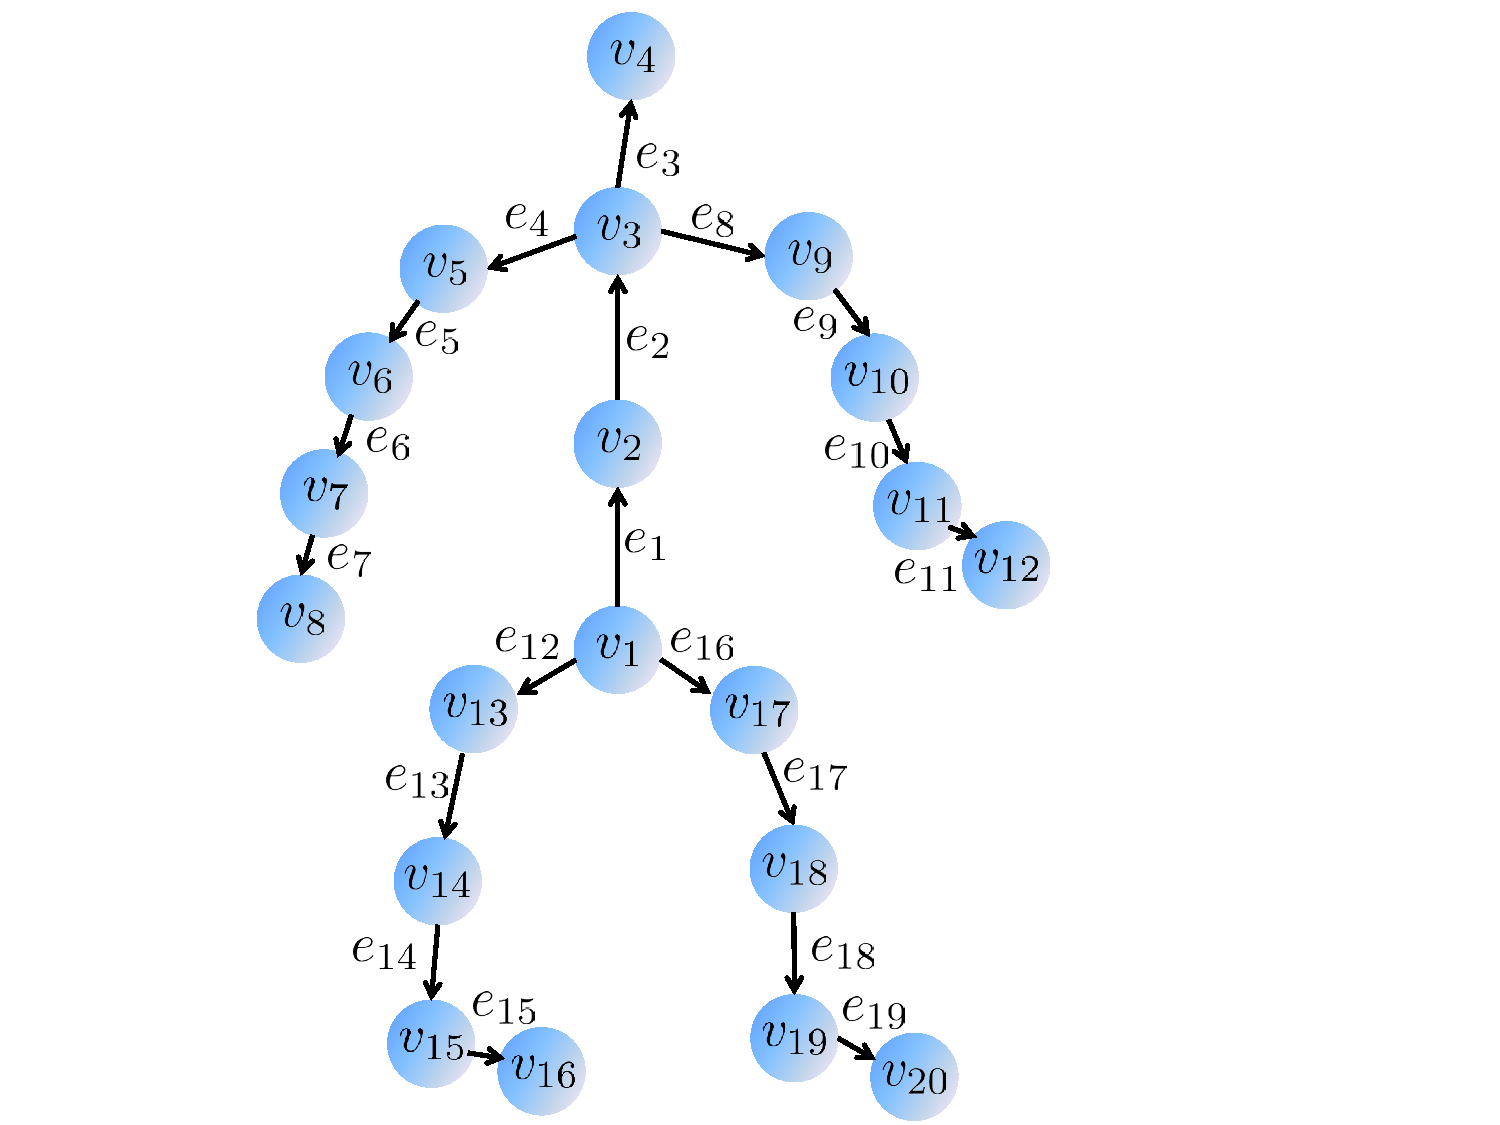
\includegraphics[width=2.3in]{skeleton.pdf}
\caption{An illustration of the skeleton. \label{fig:skeleton}}
\end{center}
\end{figure}

We compute our skeleton feature across 41 frames which includes the action center frame, 20 frames before the action center frame and 20 frames after the action center frame. Finally we concatenate all the feature vectors into a final vector.

\section{Classification Methods}
We propose two different methods for classifying interactive actions from the skeleton features.

\subsection{Generative Modeling}
Given an input video containing the action, generate a semantic desription of the action as it occurs in the video. To describe an action would mean to generate a dictionary based representation for the action. A suitable middle ground between a complete linguistic action definition and a machine-derivable description, we borrow the action vocabulary decribed in \cite{SUHA}. Accordingly, a single person action in general can be described using an \textbf{operational triplet} as follows:

\begin{equation}
<Agent-Motion-Target>
\end{equation}

where $Agent$ is the person or the body part of the person which initiates the action; $Motion$ implies the movement of the $Agent$; $Target$ can be taken to be an object or another person or his body part that is involved in the interaction. Using this terminology some simple action representations can be generated as shown below:

\begin{itemize}
\item \textbf{Handshake}: $<$Arm1 - Outstretched - Arm2$>$
\item \textbf{Kicking}: $<$Leg1 - Outstretched - Leg2$>$
\end{itemize}

It should be noted that for some actions that \textit{Agent} and \textit{Target} need not necessarily be a single person or body part but can be a collection of body parts that act on each other in a causal way. To see an example of this, consider the figure \ref{Fig:act_des}

\begin{figure}[ht]
\centering

  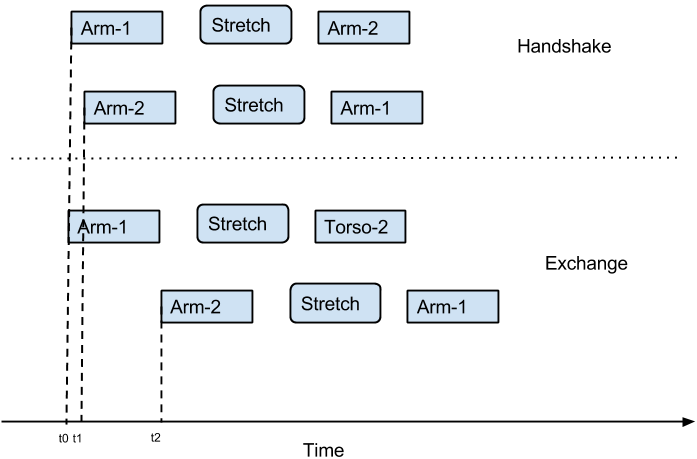
\includegraphics[scale = 0.4]{action_des.png}%
  \label{Fig:act_des}%

\end{figure}

Thus, we can see that actions that have similar semantic descriptions in terms of the operational triplet can be differentiated by means of proper temporal constraints. To look at how spatial constraints can decide the type of interaction, we incorporate that knowledge in the decision tree structure shown in figure \ref{Fig:tree}.

\begin{figure}[ht]
\centering

  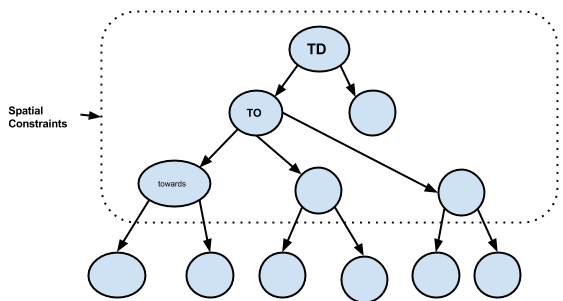
\includegraphics[scale = 0.4]{dec_tree.png}%
  \label{Fig:tree}%

\end{figure}

\subsection{Artificial Feed forward Neural Network}
We use artificial feed forward neural network with softmax activation function as its final layer to estimate conditional probability, $P(y_t|x_t,t=t_{ac})$ at time instance $t$, where $y_t$ is an action class label and $x_t$ is the skeleton features computed from $t-20$ to $t+20$ frames and $t_{ac}$ is the time instance of the action center frame. We manually localize the action center frame of the training sequences and train the model with 10 hidden layers.

In testing time, we apply the trained neural network in a time sliding window manner and obtain the conditional probability $P(y_t|x_t,t=t_{ac})$. We also apply our action center detector at each frame to obtain $P(t=t_{ac}|x_t)$. We then compute $P(y_t,t=t_{ac}|x_t)=P(y_t|x_t,t=t_{ac}) P(t=t_{ac}|x_t)$ at each frame. Finally, we compute $P(y)$ for each sequence by $\sum_{t=t_{s}}^{t_{e}} P(y_t,t=t_{ac}|x_t)$ where $t_{s}$ and $t_{e}$ are the time instance where there are sufficient number of frames to apply the neural network. The final prediction is done by $\argmax_{y} P(y)$.

\section{Experiments}

\subsection{Data Collection}

The dataset that we have is an augmented version of the already available interaction dataset which consists of 8 actions :

%\begin{figure}[ht]
%\centering
%\subfloat[Kinect Skeleton model]
%{
%  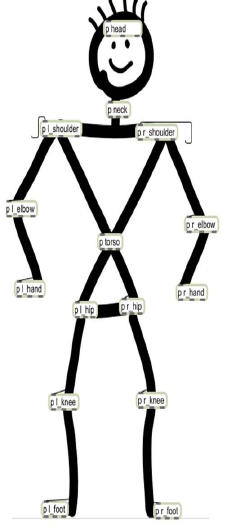
\includegraphics[scale = 0.2]{kinect_joints.png}%
%  \label{Fig:1}%
%}
%\quad
%\subfloat[Available Interaction dataset]
%{
%  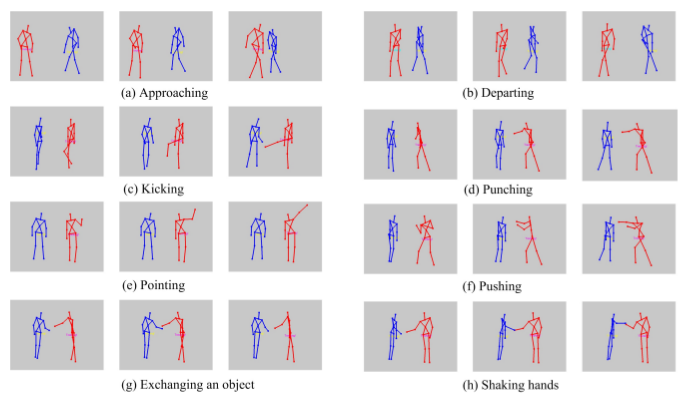
\includegraphics[scale = 0.3]{dataset.png}%
%  \label{Fig:2}%
%}
%\end{figure}

\begin{figure}[htb]
\begin{center}
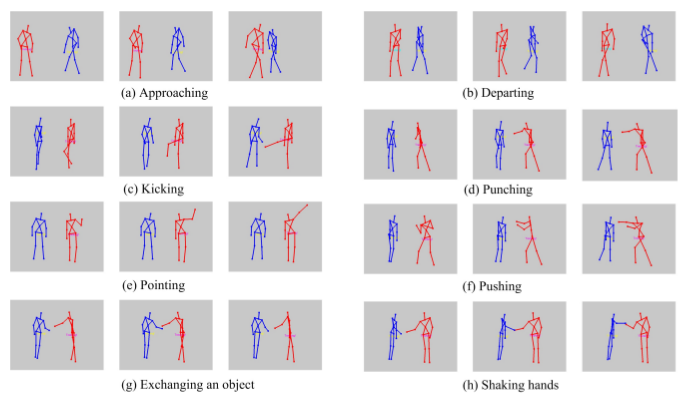
\includegraphics[width=3.4in]{dataset.png}
\caption{Available Interaction dataset \label{fig:Fig:2}}
\end{center}
\end{figure}


In addition to the available dataset, we create a new dataset of 10 different interactive actions using Kinect. The action classes we consider are summarized in Fig.\ref{fig:newactions}. For each pair of people, we collect 2 sequences per action class by switching people's locations. There are 12 sequences per action class.

\begin{figure*}[htb]
\begin{center}
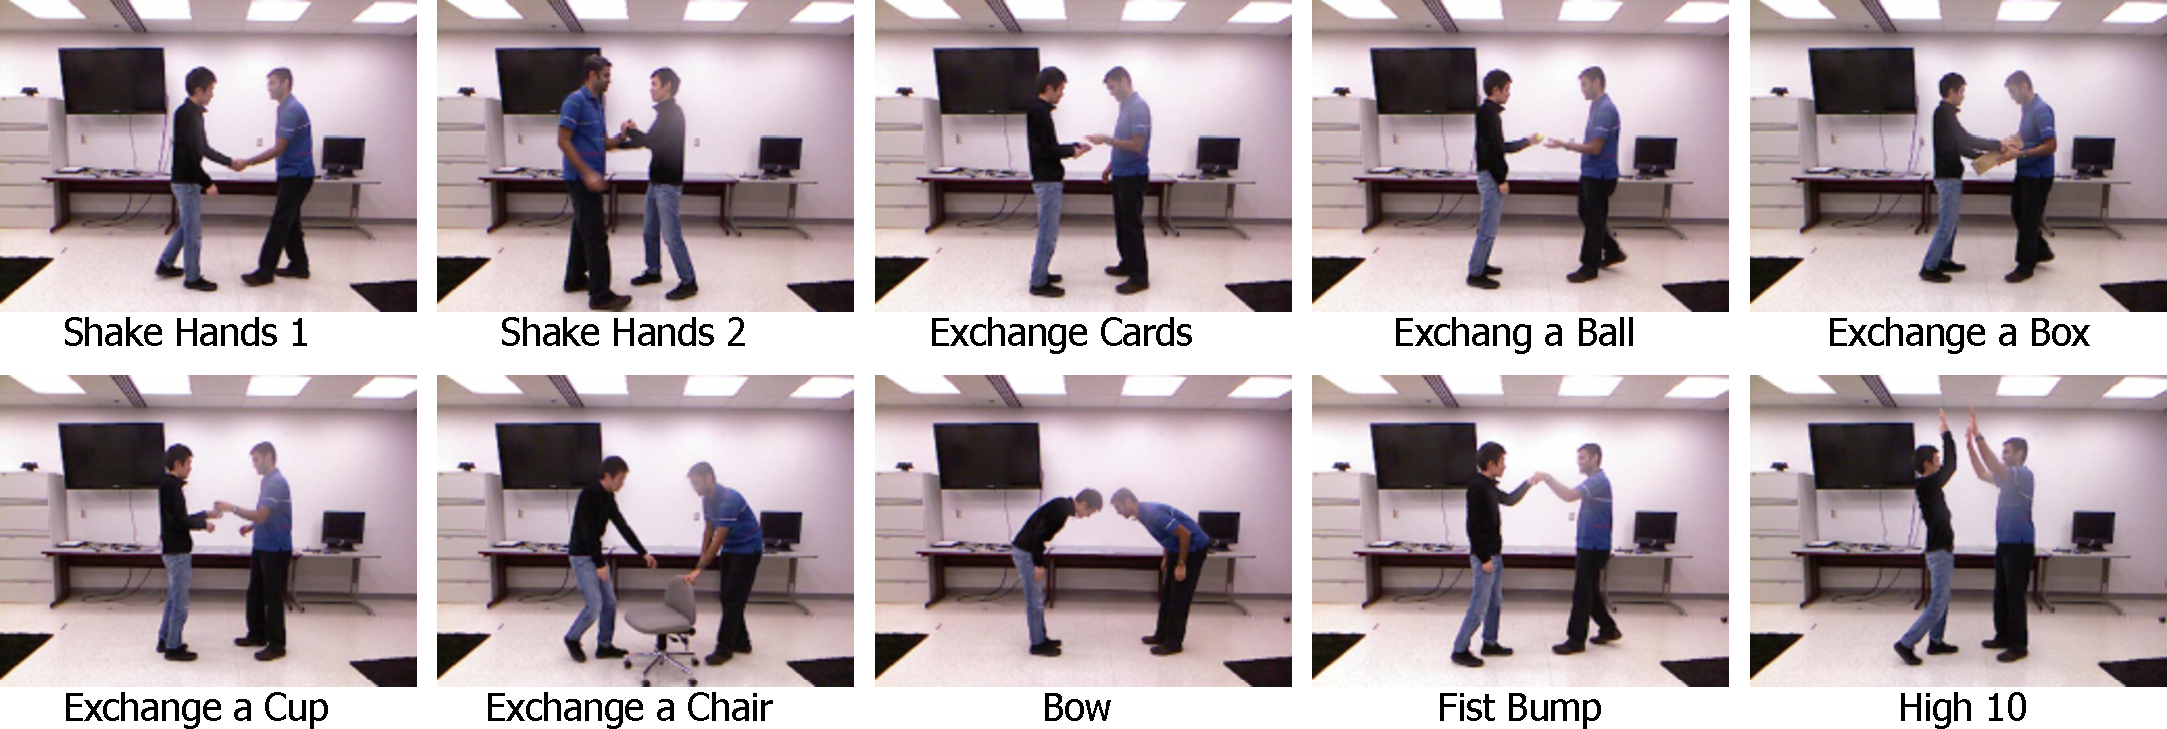
\includegraphics[width=6.8in]{newactions.pdf}
\caption{Actions in newly collected dataset \label{fig:newactions}}
\end{center}
\end{figure*}


The data is organized in the following form : 
\begin{itemize}
\item : Depth data file corresponding to frame number xxx of activity.
		
\item rgb$dummy$xxx.png: RGB data file corresponding to frame number xxx of activity.
				
\item skeleton$dummy$pos.txt: Skeleton position data

\end{itemize}
	
Skeleton data consists of 15 joints per person. Each row follows the following format.
\begin{equation*}
%\{Frame# ,PA(1),..,PA(15),PB(1),..,PB(15)\}
\end{equation*}	

where, \\
$PA(i)$ $\implies$ position of ith joint (x,y,z) for the subject A located at left \\
$PB(i)$ $\implies$ position of ith joint (x,y,z) for the subject B located at right \\
x,y and z are normalized as [0,1].	
\newline	



Steps for performing Interaction Recognition using Kinect:

Step 0 : To organize the data in the above format. To do this, we extract skeleton data from the recorded OpenNI files that comes from the Kinect sensor.

Step 1 : For each frame, we have to spatially localize each person - We are trying to figure out how to extract this information directly from the Kinect output

Step 2 : Should perform an Object Detection routine to verify if there is any sign of Object exchange

Step 3 : Based on how each joint moves in the video per frame, the activity trees are grown and the corresponding activity is detected. Primarily we want to differentiate between Object/Non-object Interactions and further classify the Non-Object Interactions into one of the Action classes that were given to us during Training. 

%The skeleton representation provides a convenient way to represent different actions in the form of Action trees. The terminal nodes of each action tree consists of the 20 joint positions. For each action, based on how different joint nodes combine to perform that action we can develop the corresponding action tree. 

\subsection{Results}




\section{Conclusion}


\begin{thebibliography}{9}

\bibitem{Vemulapalli2013}
  Raviteja  Vemulapalli,
  Felipe Arrate,
  Rama Chellappa,
  \emph{Human Action Recognition by Representing 3D Skeletons as Points in a Lie Group}.
  CVPR,
  2014.

\bibitem{SUHA} Semantic-level Understanding of Human Actions and Interactions using Event Hierarchy, Sangho Park, J.K. Aggarwal, CVPR'04

\end{thebibliography}

\end{document}
